\subsection{Results}
\label{sec:final_case_results}

The financial and computational results arise from the same experiment rather
than from separate scaling and case-study models.  The frozen empirical
universe contains 1,480 books.  In each shock path, 148 books are selected by a
fixed target seed and receive inventory-adverse orders at $t=11{,}700$ seconds.
Twenty stochastic seeds are paired across shock and no-shock paths.  The design
compares a globally constrained shared dealer with an asset-local-capacity
control and a shared-dealer-absent control.  Two per-asset reference capacities,
$L=800$ and $L=1{,}600$, are considered.  In total, the production matrix
contains 200 full-session financial paths; mechanism and rank-invariance checks
increase the total to 206 simulator executions.

\subsubsection{Computational execution and verification}

The complete matrix ran on 16 MPI ranks in \(2{:}04{:}23\), with peak resident
memory of 17.46~GiB.  It processed 25.835 billion orders and 2.049 billion
trades.  The median wall time of one full globally coupled path was 35.48~s,
with a median measured communication fraction of 32.6\%.  The corresponding
medians were 35.04~s and 34.3\% for the asset-local-capacity control, and
24.71~s and 48.0\% when the shared dealer was absent.  The larger fraction in
the last case reflects its smaller local-computation workload and should not be
read as greater absolute communication volume.

The one-rank and 16-rank preflight paths produced the identical final-state
hash \texttt{0x39ca074b1c4e5b84}.  Wall time fell from 14.049~s to 1.577~s,
corresponding to a speedup of 8.91 and parallel efficiency of 55.7\% for this
short workload.  The truncated/full-prefix certificate also passed.  Finally,
all 837 declared result artifacts were rehashed successfully.  These checks
establish that the financial comparison is invariant to the selected MPI
decomposition.

\subsubsection{Identification and mechanism}

For outcome $Y$, the primary effect is the paired difference-in-differences
estimator
\begin{equation}
\widehat{\tau}_{t}
=
\left(Y^{G,S}_{t}-Y^{G,C}_{t}\right)
-
\left(Y^{L,S}_{t}-Y^{L,C}_{t}\right),
\label{eq:final_did}
\end{equation}
where $G$ denotes global capacity, $L$ asset-local capacity, and $S$ and $C$
the shock and no-shock paths.  Common random numbers are used within each pair.
The non-target shock--control difference is exactly zero in both negative
controls at every recorded time.  Consequently, a non-zero value of
\eqref{eq:final_did} is attributable to the global inventory channel rather
than to a change in the background random stream.

The shared dealer remains active before the shock.  It requests two-sided
quotes in all 1,480 books; the minimum pre-shock resting coverage is 97.8\% at
$L=800$ and 98.0\% at $L=1{,}600$.  Utilisation is 83.7\% and 83.1\%, below the
predeclared 85\% headroom limit, with quote scales 0.326 and 0.338.  The minimum
quote scale across the full production matrix remains above the 0.05 floor.

\begin{table}[htbp]
\centering
\caption{Immediate shared-dealer response.  Brackets contain paired 95\%
confidence intervals across 20 seeds.}
\label{tab:final_mechanism}
\small
\begin{tabular}{rrrrr}
\toprule
$L$ & Exposure change & Utilisation change & Quote-scale change & Absorption \\
\midrule
800   & $5{,}384.7\ [4{,}592.1,6{,}177.2]$ & 0.00455
      & $-0.00910\ [-0.01043,-0.00776]$ & 2.02\% \\
1,600 & $6{,}621.8\ [6{,}054.7,7{,}188.9]$ & 0.00280
      & $-0.00559\ [-0.00607,-0.00511]$ & 2.52\% \\
\bottomrule
\end{tabular}
\end{table}

Table~\ref{tab:final_mechanism} confirms the mechanism in every production
seed: the shock raises global exposure and lowers the quote scale.  The tighter
capacity produces an additional quote-scale reduction of 0.00350, with paired
95\% confidence interval $[0.00254,0.00447]$ in absolute magnitude.  Requested
depth is unchanged at the one-second observation because the new scale enters
the books at the next quote-refresh boundary.  By five seconds, requested
shared depth in unshocked books has fallen by 3,370 units for $L=800$ and 1,939
units for $L=1{,}600$.  Figure~\ref{fig:final_mechanism} shows that the exposure
and quote-scale contrasts subsequently decay towards zero.

\begin{figure}[htbp]
\centering
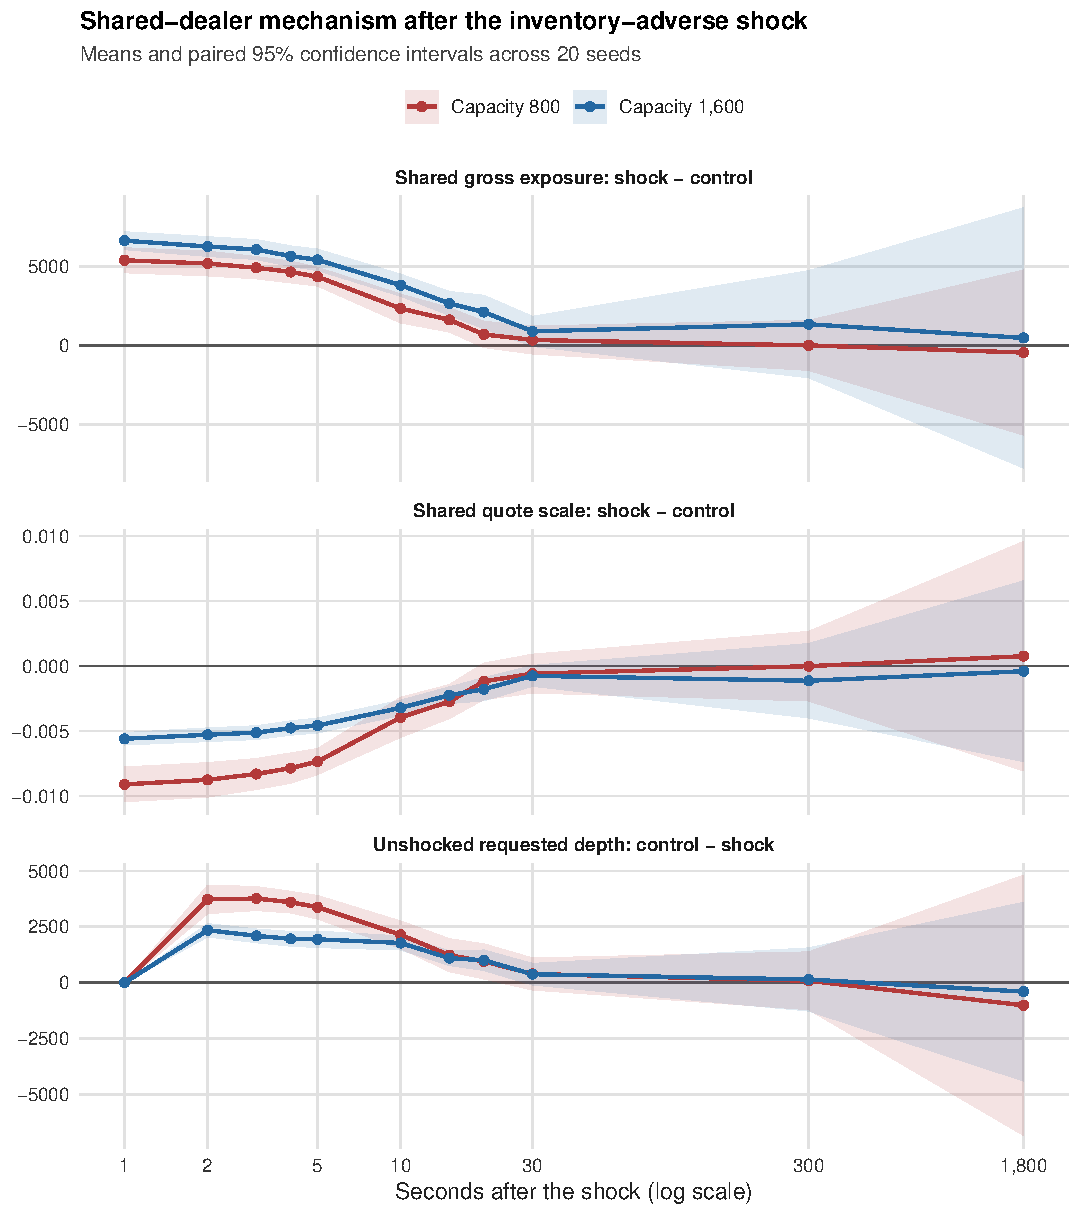
\includegraphics[width=0.83\textwidth]{docs/case-study/figures/mechanism_response.pdf}
\caption{Shared exposure, quote scale and requested depth after the shock.
Lines are seed means and shaded regions are paired 95\% confidence intervals.}
\label{fig:final_mechanism}
\end{figure}

\subsubsection{Market-wide liquidity response}

\begin{table}[htbp]
\centering
\caption{Liquidity response in unshocked books.  A positive depth value denotes
deterioration; brackets contain paired 95\% confidence intervals.}
\label{tab:final_liquidity}
\small
\begin{tabular}{rrrr}
\toprule
Horizon & $L$ & Relative top-depth change & Spread change (bp) \\
\midrule
2 s & 800   & $0.0568\%\ [0.0479,0.0656]$ & $0.00033\ [-0.00029,0.00094]$ \\
5 s & 800   & $0.0574\%\ [0.0462,0.0685]$ & $0.00135\ [-0.00176,0.00445]$ \\
5 s & 1,600 & $0.0420\%\ [0.0101,0.0738]$ & $0.00182\ [-0.00142,0.00505]$ \\
30-min mean & 800 & $0.1790\%\ [-0.2972,0.6552]$ & $-0.00115\ [-0.01431,0.01202]$ \\
30-min mean & 1,600 & $0.0108\%\ [-0.3815,0.4032]$ & $-0.00350\ [-0.01488,0.00787]$ \\
\bottomrule
\end{tabular}
\end{table}

The immediate response is statistically clear but economically small.
Top-of-book depth deteriorates by approximately 0.04--0.06\% during the first
few seconds (Table~\ref{tab:final_liquidity} and
Figure~\ref{fig:final_early_depth}).  The interval includes zero by
approximately 30 seconds.  No spread estimate in the main early or 30-minute
comparison is distinguishable from zero.  Moreover, the 30-minute depth
contrast between $L=800$ and $L=1{,}600$ is 0.168 percentage points with a
95\% confidence interval of $[-0.496,0.832]$.  The evidence therefore supports
a transient cross-asset withdrawal, but not a persistent liquidity spiral.

\begin{figure}[htbp]
\centering
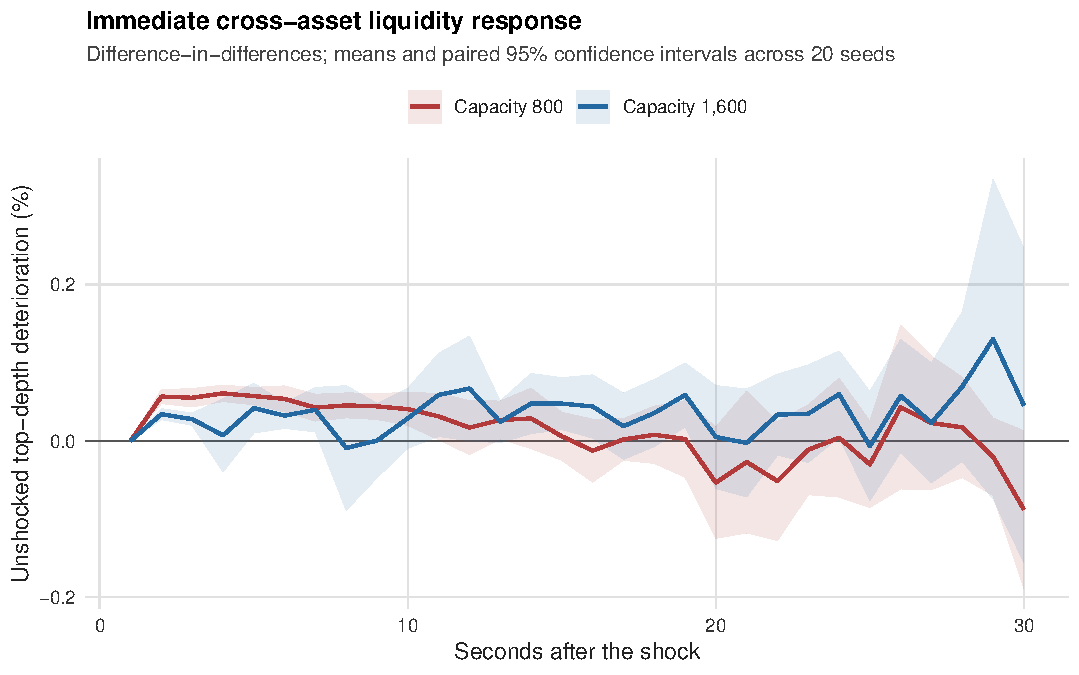
\includegraphics[width=0.83\textwidth]{docs/case-study/figures/marketwide_depth_early.pdf}
\caption{Difference-in-differences estimate of the immediate top-depth response
in unshocked books.}
\label{fig:final_early_depth}
\end{figure}

\subsubsection{Heterogeneity across liquidity clusters}

Cluster identifiers denote empirical categories and are not an ordinal
liquidity ranking.  Cluster sizes range from 70 to 266 books, so baseline depth,
spread and sample size must accompany any cluster label.  Averaged over seconds
2--10, nine of ten clusters at $L=800$ and eight of ten clusters at $L=1{,}600$
have positive depth effects whose paired intervals exclude zero.  The largest
estimates under $L=800$ occur in clusters 2 (0.157\%), 3 (0.132\%), 5
(0.124\%) and 0 (0.120\%).  The ordering is not monotone in baseline spread or
depth (Figure~\ref{fig:final_clusters}).

No cluster's 30-minute depth interval excludes zero under either capacity.
Two of 20 exploratory spread intervals exclude zero, but have opposite signs
and do not support a coherent result after accounting for multiple comparisons.
Thus the heterogeneous response is best interpreted as broad, short-lived
depth withdrawal rather than persistent cluster-specific contagion.

\begin{figure}[htbp]
\centering
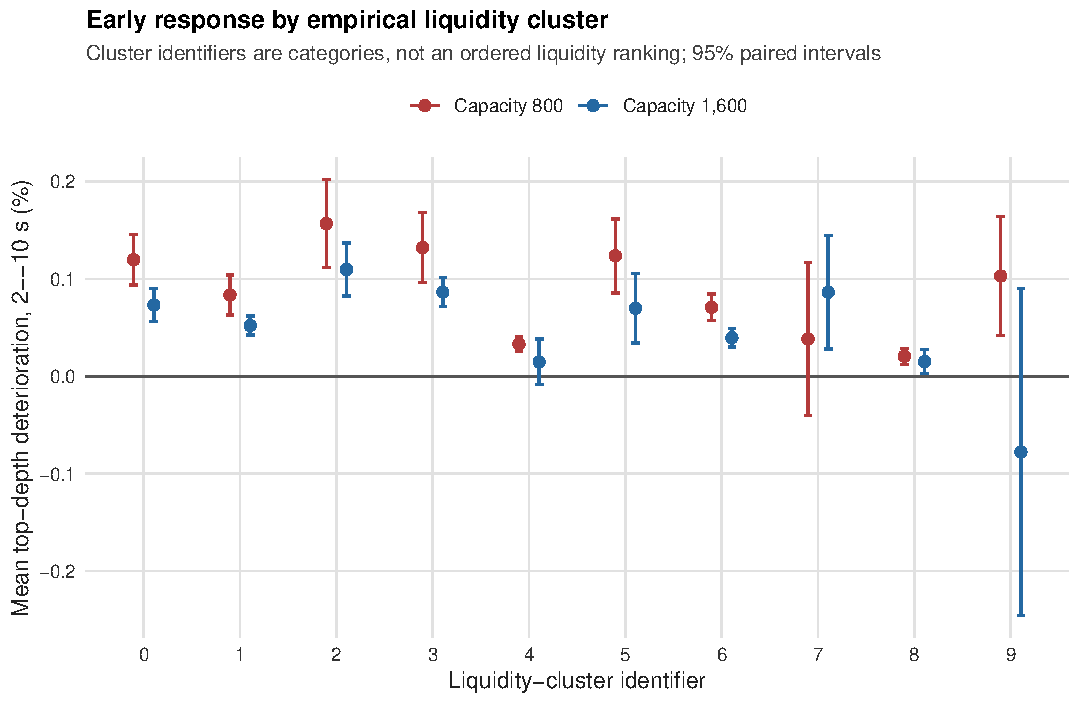
\includegraphics[width=0.83\textwidth]{docs/case-study/figures/cluster_early_response.pdf}
\caption{Mean top-depth deterioration during seconds 2--10 by empirical
liquidity cluster.  Error bars are paired 95\% confidence intervals.}
\label{fig:final_clusters}
\end{figure}

\subsubsection{Interpretation}

The experiment establishes that common inventory capacity can transmit an
adverse fill to otherwise unshocked books through a shared reduction in quoted
depth.  It also shows that the calibrated market replenishes this withdrawal
quickly.  The HPC contribution is integral to this inference: whole-book MPI
decomposition permits a deterministic, causally coupled 1,480-book
counterfactual matrix containing more than 25 billion processed orders.  The
result is evidence for a scalable and rank-independent mechanism experiment,
not historical replay or identification of an actual dealer's balance sheet.
